\def\QRCODE{TB_image_TUT.IMG.image_segmentation_histogram_clustering_pythonqrcode.png}
\def\QRPAGE{http://www.iptutorials.science/tree/master/TB_image/TUT.IMG.image_segmentation_histogram_clustering/python}
\pcorrectionsection{Python correction}

\subsection{Manual thresholding}
\subsubsection{Visual analysis of histogram}
When manually choosing a threshold value, one has to analysis the histogram (Fig. \ref{fig:histoseg:python:autothresh}).

\begin{python}
import numpy as np
import imageio
import matplotlib.pyplot as plt # plots
from skimage import filter # otsu thresholding

# read image
cells=imageio.imread('cells.png');

# display histogram
fig=plt.figure();
plt.hist(cells.flatten(), 256)
fig.show();
fig.savefig("histo.pdf");
\end{python}

\begin{figure}[htbp]
\centering\caption{Original image and its histogram.}
\subfloat[Original image.]{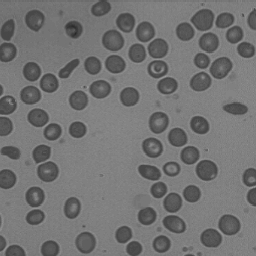
\includegraphics[width=.4\linewidth]{cells.png}}\hfill
\subfloat[Histogram.]{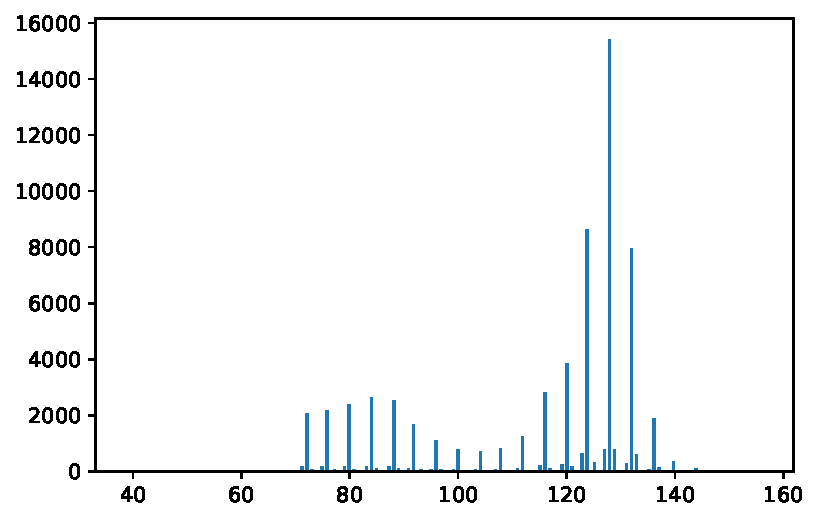
\includegraphics[width=.55\linewidth]{histo.pdf}}
 \label{fig:histoseg:python:autothresh}
\end{figure}

\subsubsection{Segmentation}
\begin{python}
fig=plt.figure();
plt.subplot(1,2,1)
plt.imshow(cells, plt.cm.gray); plt.title('Original image');
plt.subplot(1,2,2)
plt.imshow(cells>80, plt.cm.gray); plt.title('Manual segmentation');
fig.savefig("manual.pdf");
\end{python}

\subsection{Automatic thresholding}
\begin{python}
def autothresh(image):
    """ Automatic threshold method
    @param image: image to segment
    @return : threshold value
    """
    s = 0.5*(np.amin(image) + np.amax(image));
    done = False;
    while ~done:
        B = image>=s;
        sNext = .5*(np.mean(image[B]) + np.mean(image[~B]));
        done = abs(s-sNext)<.5;
        s = sNext;
    return s
\end{python}

The results are displayed using the following code (Fig. \ref{fig:histoseg:python:otsu:cells}):
\begin{python}
# Automatic threshold
s_auto= autothresh(cells);

# Otsu thresholding
s_otsu =filter.threshold_otsu(cells);

plt.figure();
plt.subplot(1,2,1)
plt.imshow(cells>s_auto, plt.cm.gray); plt.title('Automatic thresholding')
plt.subplot(1,2,2);
plt.imshow(cells>s_otsu, plt.cm.gray); plt.title('Otsu thresholding');
\end{python}

\begin{figure}[htbp]
\centering\caption{Automatic thresholding and thresholding by Otsu. Results are almost identical because threshold values are 105.3 and 105, respectively.}%
\subfloat[Automatic threshold.]{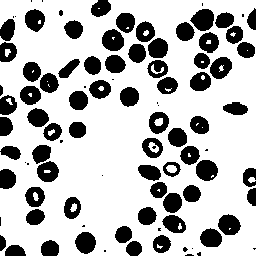
\includegraphics[width=.45\linewidth]{autothresh.png}}\hfill
\subfloat[Otsu threshold.]{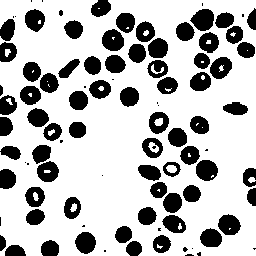
\includegraphics[width=.45\linewidth]{otsuthresh.png}}%
\label{fig:histoseg:python:otsu:cells}%
\end{figure}

\subsection{\texorpdfstring{$k$-means clustering}{k-means clustering}}
Different techniques can be found in the scikit documentation. A point cloud will first be generated, from 3 clustered cloud points. The objective is then to segment all the points into their original cluster.

\subsubsection{Imports}
\begin{python}
import numpy as np
import matplotlib.pyplot as plt
import time

from sklearn.cluster import KMeans
\end{python}


\subsubsection{Generation of point clouds}
\begin{python}
def generation(n, x, y):
    Y = np.random.randn(n, 2) + np.array([[x, y]]);
    return Y
    
points1=generation(100, 0, 0);
points2=generation(100, 3,4);
points3=generation(100, -5, -3);

pts=np.concatenate((points1, points2, points3));
plt.plot(pts[:,0], pts[:,1], 'ro');

plt.show();
\end{python}
\begin{figure}[htbp]
\centering
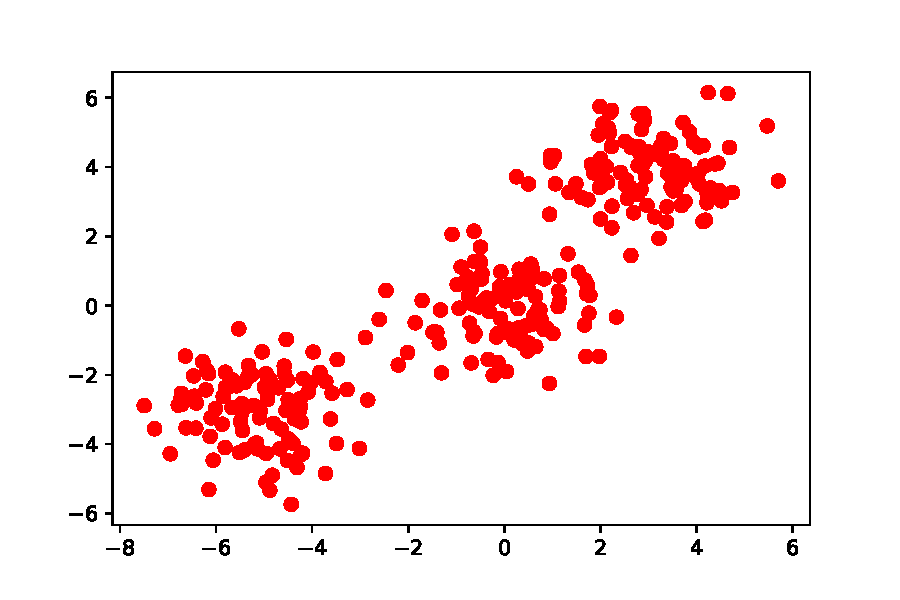
\includegraphics[width=10cm]{points.pdf}
\caption{Point cloud.}
\end{figure}

\subsubsection{\texorpdfstring{$k$}{k}-means clustering}
\begin{python}
n=3; # number of clusters

# k-means initialization
k_means = KMeans(init='k-means++', n_clusters=n, n_init=10)
t0 = time.time(); # computation time
k_means.fit(pts); # kmeans segmentation

t_batch = time.time() - t0;

# retrieve results
k_means_labels = k_means.labels_;
k_means_cluster_centers = k_means.cluster_centers_;

# plot
fig = plt.figure()
colors = ['#4EACC5', '#FF9C34', '#4E9A06']

# k-means
# zip agregates values two by two
for k, col in zip(range(n), colors):
    my_members = k_means_labels == k
    cluster_center = k_means_cluster_centers[k]
    
    # display points
    plt.plot(pts[my_members, 0], pts[my_members, 1], 'w',
            markerfacecolor=col, marker='.')
            
    # display centroid
    plt.plot(cluster_center[0], cluster_center[1], 'o', 
				 markerfacecolor=col, markeredgecolor='k', 
				 markersize=6)
plt.title('KMeans')
plt.show()
fig.savefig("kmeans.pdf");
\end{python}

%\begin{figure}[htbp]
%\centering
\centerline{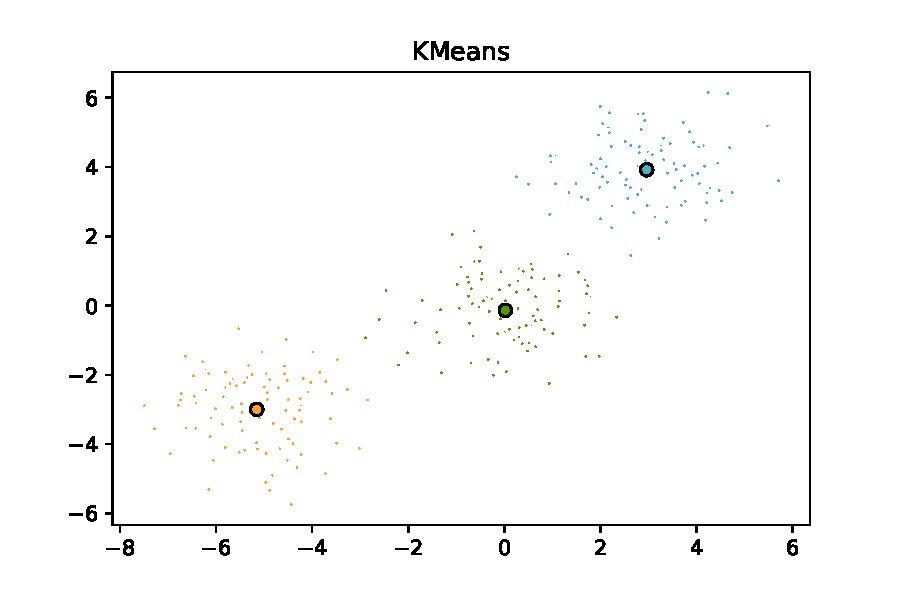
\includegraphics[width=10cm]{kmeans.pdf}}
%\end{figure}

\subsection{Color image segmentation}
Three different colors can be observed in the image. The objective is to separate the 3 colors with the help of the K-means algorithm. Thus, the segmentation is performed in the RGB color space, and each pixel is represented by a point in this 3D space.
Initialization steps are identical to previous code. The data is converted from a color image (of size $(n,m,3)$) to a vector (of size $(n\times m, 3)$), done by the \pinline{reshape} function of numpy. 

\begin{python}
# load color image
cells=imageio.imread('Tv16.png');
[nLines,nCols,channels] = cells.shape
# reshape data
data = np.reshape(cells, (nLines*nCols, channels));
k_means.fit(data);
# convert result to an image
# as we got labels, we expand the dynamic (multiply by 70)
segmentation = 70*np.reshape(k_means.labels_, (nLines, nCols));

fig=plt.figure();
plt.imshow(segmentation, cmap=plt.cm.gray);
imageio.imwrite("segmentation_kmeans.png", segmentation);
\end{python}

\begin{figure}[htbp]
\centering\caption{Segmentation result.}%
\subfloat[Original image.]{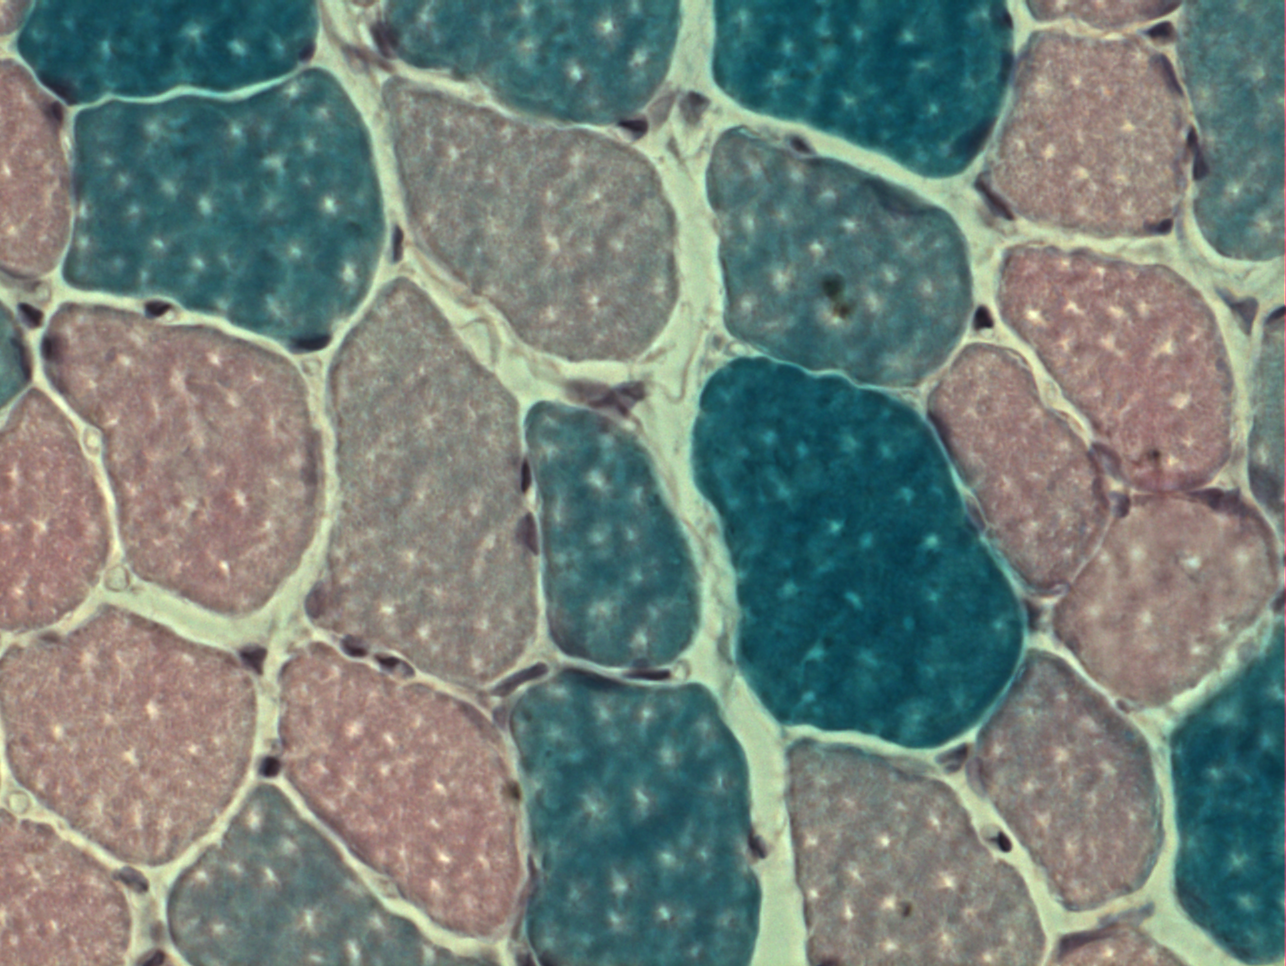
\includegraphics[width=5cm]{Tv16.png}}
\hspace{1cm}
\subfloat[Segmented.]{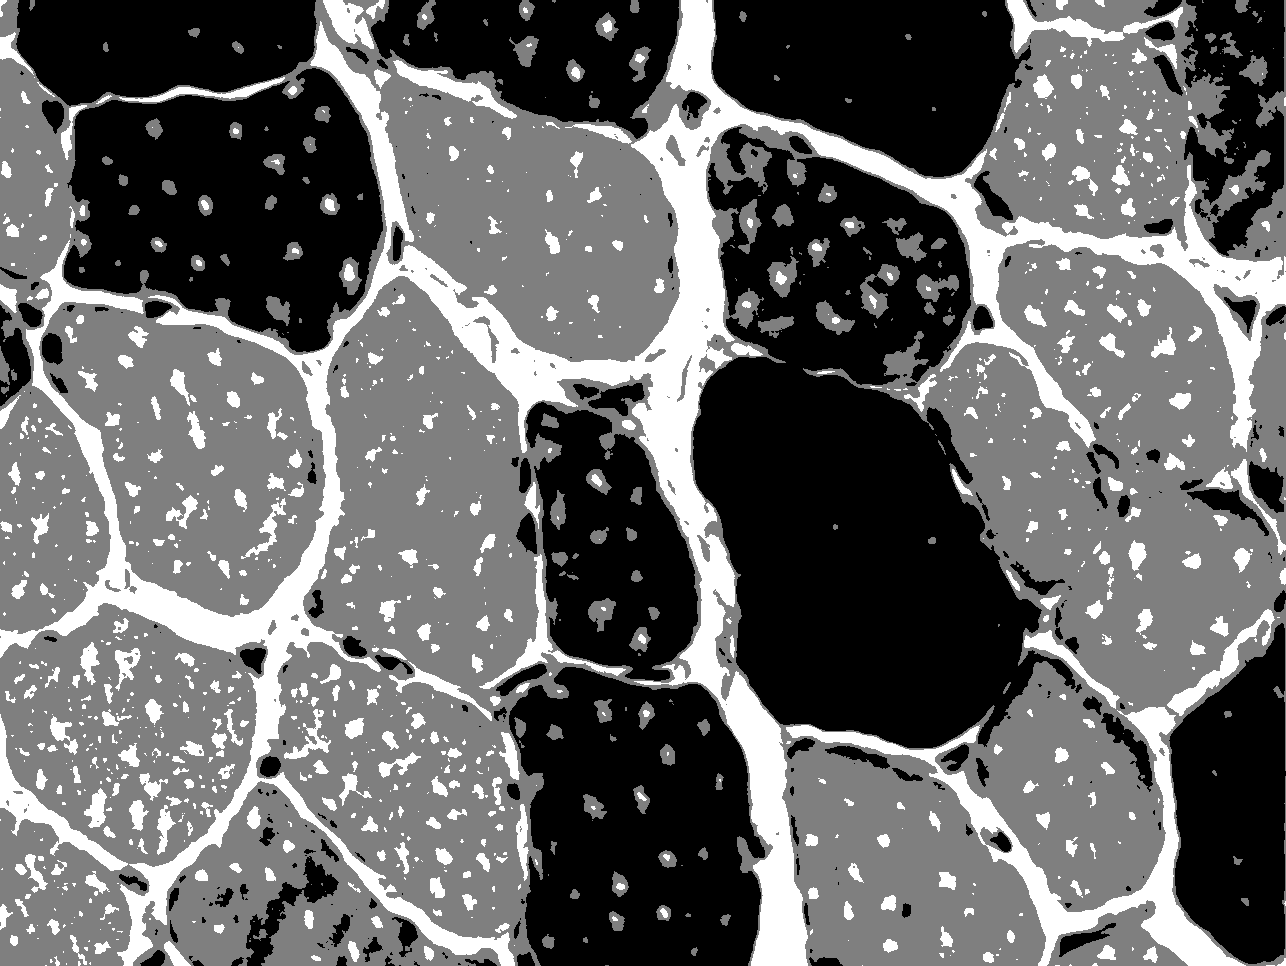
\includegraphics[width=5cm]{segmentation_kmeans.png}}%
\label{fig:histoseg:python:segmentation}%
\end{figure}

\vspace*{-6pt}

\subsubsection{3D scatter plot}
This is a method to display colors in the RGB cube. This method is really slow, depending on your GPU.

\begin{python}
from mpl_toolkits.mplot3d import Axes3D # 3D scatter plot
# plot
colors = ['#4EACC5', '#FF9C34', '#4E9A06']
        
fig = plt.figure()
ax = fig.add_subplot(111, projection='3d')

# Plot scatter points
for k, col in zip(range(n), colors):
    my_members = k_means_labels == k
    cluster_center = k_means_cluster_centers[k]
    ax.scatter(data[my_members, 0], data[my_members, 1], 
					data[my_members, 2], c=col)
    ax.scatter(cluster_center[0], cluster_center[1], 
					cluster_center[2], s=30, c=col)
\end{python}
